% ======================================================================
%  Trading in the Dark: Deep Reinforcement Learning for Jane Street's
%  Figgie -- full paper
%
%  Compile:  tectonic main.tex   (or pdflatex + bibtex + pdflatex x2)
%  Figures:  pgfplots reads data/*.dat; regenerate with make_figures.py
% ======================================================================
\documentclass[11pt]{article}

\usepackage[T1]{fontenc}
\usepackage{lmodern}
\usepackage[utf8]{inputenc}
\usepackage[a4paper,margin=1in]{geometry}
\usepackage{amsmath,amssymb}
\usepackage{microtype}
\usepackage{booktabs}
\usepackage{graphicx}
\usepackage{xcolor}
\usepackage{caption}
\usepackage{subcaption}
\usepackage{enumitem}
\usepackage{float}
\usepackage{algorithm}
\usepackage{algpseudocode}
\usepackage{natbib}
\usepackage{pgfplots}
\usepackage{tikz}
\usetikzlibrary{arrows.meta,positioning,calc,shapes.geometric}
\usepackage[colorlinks=true,linkcolor=figgienavy!60,citecolor=figgiegreen,urlcolor=figgiegray]{hyperref}

% ----------------------------------------------------------------------
% Palette (colorblind-safe; plotted data + prose share it)
% ----------------------------------------------------------------------
\definecolor{figgienavy}{HTML}{1F3B73}
\definecolor{figgieteal}{HTML}{2A9D8F}
\definecolor{figgieorange}{HTML}{E76F51}
\definecolor{figgiegray}{HTML}{8D99AE}
\definecolor{figgiegold}{HTML}{E9C46A}
\definecolor{figgiegreen}{HTML}{33658A}

\pgfplotsset{compat=1.17}

% ----------------------------------------------------------------------
\title{\textbf{Trading in the Dark: Deep Reinforcement Learning for Jane Street's Figgie}}

\author{Henry Hudepohl\\\small\texttt{henryhudepohl@g.ucla.edu}}

\date{\today}

\emergencystretch=2em
\begin{document}
\maketitle

% ----------------------------------------------------------------------
\begin{abstract}
\noindent
We study a deep-reinforcement-learning (DRL) agent for \emph{Figgie}, Jane
Street's hidden-information negotiation card game. Figgie combines a small
hidden ``world'' (a suit-count assignment drawn from only twelve
possibilities) with general-sum, multi-player, continuous-time trading, so
the dominant skill is signal extraction and price discovery rather than
planning depth. We build a discretized simultaneous-move engine, maintain an
\emph{exact} strategy-free posterior over the hidden assignment (a dynamic
program over deals, validated to ECE $0.02$--$0.08$ against simulator truth),
and train an AlphaZero-style search agent, information-set Monte Carlo tree
search (IS-MCTS) with neural policy/value/belief priors, via population-based
self-play. Against three random bots the resulting agent wins $95$--$97\%$ of
rounds (mean round delta $+\$126\pm5$) and outperforms every baseline in a
fixed mixed pool. Our headline finding is a \emph{saturation within our
evaluation setup}: the random-pool result plateaus at M4 parity
($+\$109.8\to+\$127.8$ across our two major ablations, with the gain
concentrated in the first neural-prior step), and additional
machinery (a trade-history attention model, a learned behavior-conditioned
belief head, Bayes-combining that belief into the observation, and value-head
recalibration) does not move the random-pool metric. The same machinery
\emph{does} help against a mixed pool of behavior-driven bots ($+5.25$ from the
learned belief, another $+5.75$ from Bayes-combining it), revealing that
behavior conditioning only pays off when opponents themselves encode
information in their actions. We also report an honest negative result: a
correctly implemented bundle-quote mechanism (verified by four engine
invariants) is spammed by the policy (63\% of turns) but almost never filled
(1.4\% of trades), because our opponents do not price information. All results
are relative to the released fixed opponent pools and action abstraction; we
claim no human comparison, and the only external baselines are hand-coded
heuristics and the search-free Figgie-Lite CFR policy agent
(\S\ref{sec:cfr}). All code, checkpoints, and
seed-configurable evaluations are released.
\end{abstract}

% ----------------------------------------------------------------------
\section{Introduction}
\label{sec:intro}

Multi-agent trading games are an attractive frontier for reinforcement
learning because they combine imperfect information, general-sum incentives,
and continuous-time interaction, precisely the assumptions that classic
self-play algorithms were not designed for \citep{silver2018alphazero,
lanctot2017unified}. \emph{Figgie}, a card game created by Jane Street to
simulate market microstructure \citep{figgierules}, is a compact and
reproducible instance of this difficulty: a $4$--$5$ player, ~$4$-minute
negotiation in which the only hidden ``facts of the world'' are a $12$-way
suit-count assignment and the distribution of cards in opponents' hands, and
in which nearly all of the skill is extracting beliefs from \emph{others'
behavior} while concealing one's own.

This paper reports the methodology and results of a complete DRL pipeline for
Figgie: an exact belief tracker, an information-set search agent, a compact
neural network, and a population-based self-play loop. We make the following
contributions.

\begin{enumerate}[leftmargin=1.5em]
  \item \textbf{A rule-complete, discretized environment and exact belief
  tracker.} We formalize Figgie as a simultaneous-move game over $120$
  discrete ticks and maintain the posterior over the hidden assignment
  \emph{exactly} by dynamic programming, with consistency encoded as a
  cumulative-drawdown constraint on each opponent's hand. The posterior is
  calibrated to simulator ground truth (assignment ECE $0.02$--$0.04$; goal
  marginal ECE $0.04$--$0.08$; goal-suit argmax $39$--$41\%$ vs.\ $25\%$
  chance).
  \item \textbf{An IS-MCTS agent with neural priors trained by population
  self-play.} Belief-consistent determinized search (as in the ReBeL line
  \citep{brown2020rebel}) with PUCT selection, a 4-player value head, a
  learned belief head, and a history pathway (flat MLP, later single-head
  self-attention). Against three random bots it wins $95$--$97\%$ of rounds
  with mean round delta $+\$126\pm5$.
  \item \textbf{A saturation finding.} The random-pool headline plateaus at
  M4 parity; gains from $+109.8$ to $+123.3$ come from the first
  neural-prior step, and later modules (attention history, learned belief,
  Bayes-combine, value recalibration) do not move it. The same modules do
  move the mixed-pool result, giving a consistent picture: \emph{behavior
  conditioning only helps against behavior-driven opponents}.
  \item \textbf{Two honest negative results.} (i)~The scalar value head is
  essentially uninformative in the liquid random-pool regime
  (corr$\approx0$), yet a recalibration (P1v) restores top-bin calibration;
  (ii)~bundle quotes are mechanism-correct but the policy spams non-crossing
  bids rather than using them profitably.
  \item \textbf{An external, search-free baseline.} A two-player zero-sum
  reduction (Figgie-Lite) is solved exactly with CFR, bounding the reduced-game
  exploitability of our approach ($\varepsilon \approx 0.04$--$0.09$, near
  zero), and the resulting policy agent -- no search, no neural net -- wins
  $+\$46.6$ in the random pool, isolating the value of search and neural
  priors ($\S\ref{sec:cfr}$).
  \item \textbf{Verified, calibrated engineering.} The engine is checked
  against seven formal properties by a QuickCheck-style suite of 48 passing
  assertions, and the belief tracker, value head, and training stability are
  validated against simulator ground truth (\S\ref{sec:vv}).
\end{enumerate}

\section{Related work}
\label{sec:related}

\paragraph{Search with self-play priors.} AlphaGo Zero showed that a fully
self-contained self-play pipeline with a deep value prior can reach
superhuman planning \citep{silver2017alphagozero}; AlphaZero generalized the
recipe across Go, chess, and shogi \citep{silver2018alphazero}, and MuZero
removed the hand-coded environment model \citep{schrittwieser2020muzero}.
These methods assume perfect information, two-player, zero-sum play, all three
of which Figgie violates. The imperfect-information literature relaxes each
assumption in turn: deep counterfactual regret minimization learns from
self-play in imperfect information \citep{heinrich2016fsp}; DeepStack pairs
deep value networks with localized counterfactual evaluation for heads-up
no-limit poker \citep{moravcik2017deepstack}; Pluribus extends superhuman play
to six-player, general-sum no-limit poker with search over public states and
averaged opponent ranges \citep{brown2019pluribus}; and ReBeL unifies search
and self-play for imperfect-information games by learning value and range
models over public states \citep{brown2020rebel}. Our belief-consistent
IS-MCTS \citep{cowling2012ismcts} occupies the same design region at two
orders of magnitude less compute, which is the point of Figgie as a
reproducible benchmark.

\paragraph{Multi-player negotiation and opponent modeling.} General-sum,
multi-agent environments can exhibit cycling and incentive complexity that
pure self-play does not resolve \citep{lanctot2017unified}; population-based
training with evaluation against fixed pools is the standard mitigation
\citep{bansal2018emergent, lanctot2017unified}. Suphx masters four-player
mahjong under a similar hidden-world, hidden-hand structure
\citep{li2020suphx}. Diplomacy (a seven-player negotiation game with
order-writing) reached human level by combining language models with search
over joint orders \citep{bakhtin2022diplomacy}, and end-to-end learning for
negotiation dialogues shows that agents can extract value from mixed-motive
bargaining \citep{lewis2017deal}. Figgie is unusual among these benchmarks in
that its hidden state is tiny (twelve assignments) while nearly all skill lies
in reading opponents' \emph{behavior} rather than in search depth; we
therefore draw most directly on the opponent-modeling literature
\citep{willemsen2021opponent} and adopt OpenSpiel's conventions for
reproducible game experiments \citep{lanctot2019openspiel}.

\paragraph{Verification and calibration.} Because our claims concern a
simulator we wrote and learned components that must be calibrated, we adopt
two complementary disciplines. Property-based random testing in the QuickCheck
tradition \citep{claessen2000quickcheck} verifies the engine's formal
invariants on every commit, and we report calibration of learned probability
outputs with reliability diagrams \citep{niculescu2005probabilities} and the
expected calibration error \citep{naeini2015obtaining, guo2017calibration}.
Section~\ref{sec:vv} details the specific properties and measurements.

\section{Background: the game of Figgie}
\label{sec:background}

\paragraph{Rules.} Figgie is played by $4$ or $5$ players, each starting with
$\$350$. Players ante an equal share to form a $\$200$ pot. A deck of $40$
cards contains four suits, two black (spades, clubs) and two red (hearts,
diamonds), with suit sizes $8$, $10$, $10$, $12$; the suit$\to$size
assignment is drawn uniformly and \emph{hidden until the round ends}. The
\emph{goal suit} is always the same \emph{color} as the $12$-card suit; within
that color, the goal suit itself contains $8$ or $10$ cards. All non-goal
suits are worthless. Cards are dealt evenly and randomly. During a $4$-minute
trading phase players post bids and offers and buy and sell suits from one
another; cards of a suit are fungible. At round end each player earns
$\$10$ per goal-suit card in hand, and the remainder of the pot is split
among the player(s) holding the most goal-suit cards (ties split). The
tournament objective is cumulative money across rounds.

\paragraph{Why it is hard.} Three structural facts drive our design
choices.

\begin{enumerate}[leftmargin=1.5em]
  \item \textbf{Tiny hidden state, big deduction problem.} The only hidden
  ``world facts'' are the assignment $a \in \mathcal{A}$ (just $12$ possible
  assignments) and opponents' hands. The agent's own hand prunes impossible
  assignments immediately, so the hidden state is small enough that the belief
  can be computed \emph{exactly} rather than sampled. What makes the game hard
  is not the state space but the fact that \emph{negotiation is the game}:
  most information is conveyed by what opponents choose to buy and sell.
  \item \textbf{General-sum, multi-player, simultaneous.} AlphaZero's
  perfect-information, two-player, zero-sum assumptions do not transfer
  \citep{silver2018alphazero}. There is no well-defined exploitability
  measure, and pure self-play can cycle; we therefore use population-based
  training and empirical pool domination as our success criterion.
  \item \textbf{Asymmetric risk in dumping.} Holding junk is free (no
  hand-size limit), but discarding a wrongly suspected goal card is a real
  loss. With a weak hand prior ($P(\text{true goal}) \ge 0.5$ in only
  $\sim$17\% of rounds), naive sell rules destroy the agent's own goal cards.
  This motivated our buy-only action restriction ($\S$\ref{sec:env}).
\end{enumerate}

% ----------------------------------------------------------------------
\section{Method}
\label{sec:method}

Figure~\ref{fig:arch} summarizes the full data flow as an overview before we
detail each component: the engine and exact belief produce the observation;
the network supplies policy\slash value\slash belief priors; IS-MCTS
determinizes belief-consistent worlds and returns a policy $\pi$; and the
training loop (population mixture, replay, loss) returns gradients to the
network.

\begin{figure}[t]
\centering
\resizebox{\textwidth}{!}{%
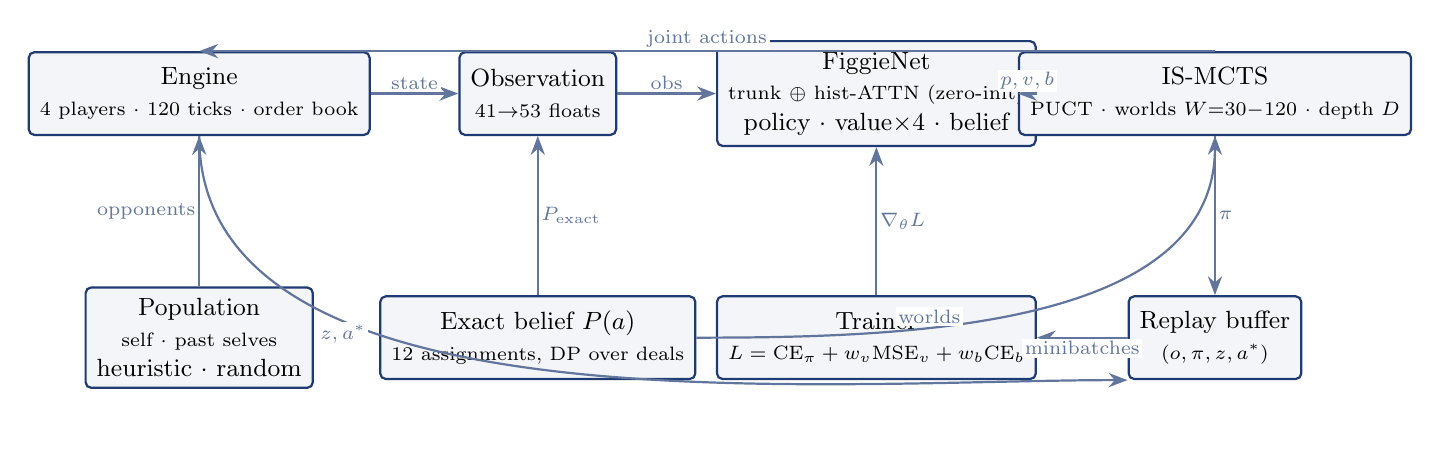
\begin{tikzpicture}[
  box/.style={draw=figgienavy, thick, rounded corners=2pt, fill=figgienavy!5,
    align=center, font=\small, minimum height=1.05cm, inner sep=4pt},
  small/.style={draw=figgiegray, rounded corners=2pt, align=center,
    font=\scriptsize, inner sep=3pt},
  lbl/.style={font=\scriptsize, fill=white, inner sep=1pt},
  arr/.style={-{Stealth[length=2.4mm]}, thick, figgienavy!70},
]
\node[box] (env) at (0,0) {Engine\\\scriptsize 4 players $\cdot$ 120 ticks $\cdot$ order book};
\node[box] (obs) at (4.3,0) {Observation\\\scriptsize 41$\to$53 floats};
\node[box] (net) at (8.6,0) {FiggieNet\\\scriptsize trunk $\oplus$ hist-ATTN (zero-init)\\policy $\cdot$ value$\times4$ $\cdot$ belief};
\node[box] (search) at (12.9,0) {IS-MCTS\\\scriptsize PUCT $\cdot$ worlds $W{=}30{-}120$ $\cdot$ depth $D$};
\node[box] (belief) at (4.3,-3.1) {Exact belief $P(a)$\\\scriptsize 12 assignments, DP over deals};
\node[box] (pop) at (0,-3.1) {Population\\\scriptsize self $\cdot$ past selves\\heuristic $\cdot$ random};
\node[box] (buf) at (12.9,-3.1) {Replay buffer\\\scriptsize $(o,\pi,z,a^*)$};
\node[box] (train) at (8.6,-3.1) {Trainer\\\scriptsize $L=\mathrm{CE}_\pi+w_v\mathrm{MSE}_v+w_b\mathrm{CE}_b$};
% --- main pipeline ---
\draw[arr] (env.east) -- node[lbl,above] {state} (obs.west);
\draw[arr] (obs.east) -- node[lbl,above] {obs} (net.west);
\draw[arr] (net.east) -- node[lbl,above] {$p,v,b$} (search.west);
\draw[arr] (search.north) to[out=180,in=0,looseness=1.1]
  node[lbl,above,pos=0.5] {joint actions} (env.north);
% --- belief ---
\draw[arr] (belief.north) -- node[lbl,right] {$P_{\mathrm{exact}}$} (obs.south);
\draw[arr] (belief.east) to[out=0,in=-90,looseness=0.9]
  node[lbl,above,pos=0.35] {worlds} (search.south);
% --- population ---
\draw[arr] (pop.north) -- node[lbl,left] {opponents} (env.south);
% --- training loop ---
\draw[arr] (search.south) -- node[lbl,right] {$\pi$} (buf.north);
\draw[arr] (env.south) to[out=-90,in=180,looseness=0.8]
  node[lbl,below,pos=0.3] {$z,a^*$} (buf.south west);
\draw[arr] (buf.west) -- node[lbl,below] {minibatches} (train.east);
\draw[arr] (train.north) -- node[lbl,right] {$\nabla_\theta L$} (net.south);
\end{tikzpicture}}%
\captionsetup{justification=raggedright}
\caption{\textbf{System architecture.} The engine and exact belief produce
the observation; the network supplies policy\slash value\slash belief priors;
IS-MCTS samples belief-consistent worlds and emits a policy $\pi$; the
training loop draws opponents from a population mixture, stores trajectories,
and returns gradients (\S\ref{sec:env}--\S\ref{sec:train}).}
\label{fig:arch}
\end{figure}

\subsection{Environment and action abstraction}
\label{sec:env}

We model the continuous trading phase as a \emph{simultaneous-move} game over
$T=120$ discrete ticks (2 s each), approximating the 4-minute clock. The
market is an order book: per suit, each player may rest a bid (maximum price
they will pay) or ask (minimum price they will accept). A trade executes when
a bid meets or exceeds an ask; execution occurs at the \emph{resting}
quote's limit price, and conflicts are resolved deterministically by player
index. Trades move one card per quote.

The discrete action set per tick is: \textsc{Pass}, \textsc{PostBid}$(S,b)$,
\textsc{PostAsk}$(S,b)$ on a coarse price grid $b \in \{6,12,18,24\}$,
\textsc{AcceptBid}, \textsc{AcceptAsk}, and \textsc{Withdraw}. Our baseline
regime is \emph{buy-only}: the agent may pass, accept an opposing ask, or
post a bid, giving $21$ actions ($1 + 4\text{ suits} \times (1 + 4)$); selling
is disabled because of the asymmetric-risk observation above. An extension
(P1b, $\S$\ref{sec:bundle}) adds combined two-suit bundle bids, growing the
action space to $45$ and the observation to $53$ floats.

Each tick every agent submits an action simultaneously; the engine resolves
crossing quotes, updates the book, and advances time. Full money conservation
and trade legality are enforced by property tests (48 passing tests total,
including payout conservation and the four bundle invariants;
\S\ref{sec:vv}).

\subsection{Exact belief tracking}
\label{sec:belief}

At any moment the only genuinely hidden facts are the assignment $a$ and the
opponents' hands. Because there are just twelve possible assignments, we can
afford to \emph{enumerate them exactly} instead of approximating with a
particle filter or heuristic scores: rather than sampling a belief, we count,
for each of the twelve worlds, how many ways the unseen cards could be split
consistent with everything observed. That count is the posterior weight; no
sampling noise enters it. Formally:

Let $\mathcal{A}$ be the set of assignments (suit$\to$size) consistent with
the revealed count pattern $8/10/10/12$; $|\mathcal{A}|=12$ after accounting
for the duplicate $10$s. A \emph{world} is an assignment $a$ together with a
distribution of the remaining cards into players' hands. The posterior
\[
  P(a \mid \text{history}) \propto P_{\text{prior}}(a) \cdot N_{\text{consistent}}(a),
\]
where $N_{\text{consistent}}(a)$ counts, under the multinomial deal
distribution, the number of hand-splits consistent with $a$ \emph{and} with
every observed trade. A world is consistent iff no observed sale drove its
seller's hand negative; per (player, suit), this reduces to the requirement
that the seller's initial holding in that suit exceed the maximum cumulative
drawdown seen in the trade history. $N_{\text{consistent}}(a)$ is computed
\emph{exactly} by a dynamic program over deals, weighting each suit split by
its multinomial multiplicity. This avoids the resampling noise and bootstrap
collapse of a particle filter while remaining cheap: the assignment space has
only $12$ elements. Particles are retained solely to sample consistent worlds
for search determinizations.

We validated the tracker against simulator ground truth on logged rounds
(M1): assignment ECE $0.03$ against heuristic opponents / $0.02$ against
random; goal-marginal ECE $0.08/0.04$; goal-suit argmax $39$--$41\%$ versus
$25\%$ chance (\S\ref{sec:vv}). The strategy-free model is mildly
overconfident and, because
drawdown constraints rarely bind against our opponents, hugs the hand prior.
Two consequences shaped the later design: (i) the posterior is well calibrated
and safe to feed to search, but (ii) it is \emph{weakly informative}, and real
belief gains must come from conditioning on \emph{behavior} (P2, $\S$\ref{sec:beliefhead}).

\subsection{Neural network}
\label{sec:net}

FiggieNet takes the $41$-float observation vector (own hand per suit, best
bid/ask per suit, own and opponent cash, elapsed time, goal-suit marginals,
the $12$-way exact posterior, own-bid flags, per-suit trade counts) and, in
later variants, a trailing window of the last $8$ trades (5 floats per trade).
The trunk is a two-layer ReLU MLP ($128$ units each, $\sim$40k parameters,
CPU). The \emph{history pathway} is a parallel branch over the trade window, a flat
MLP in P1 or a single-head self-attention projection ($5\to32$, mean-pooled) in
P2, whose output is added to the trunk as a \emph{zero-initialized residual},
so warm-started checkpoints are unaffected until the branch learns. Three heads share the trunk:

\begin{itemize}[leftmargin=1.5em]
  \item \textbf{Policy head}: logits over the masked legal action set
  ($21$, later $45$).
  \item \textbf{4-player value head}: predicts the normalized settle delta
  ($z = \text{settle}/50$) for \emph{self and each opponent}, trained by MSE
  on all four. The final layer is zero-initialized so that warm-starts remain
  exact. An ablation showed this head carries genuine search signal: zeroing
  the value head in P1 collapses the random-pool result from $+\$111$ to
  $+\$49.9$.
  \item \textbf{Belief head} (P2): a $12$-way softmax over assignments,
  trained by cross-entropy against the true assignment recorded during
  self-play. It is \emph{decoupled} from the observation encoding: the obs
  always contains the exact strategy-free posterior, and the belief head only
  produces a prior that re-weights search's world sampling
  ($\S$\ref{sec:beliefhead}).
\end{itemize}

\subsection{Search: information-set MCTS with neural priors}
\label{sec:search}

At each decision point the agent does not know the true world. We use
\emph{determinized} IS-MCTS \citep{cowling2012ismcts}: each simulation
samples a consistent world from the belief tracker and plays a shared tree
over the \emph{information-set} (public) state. Our own actions are selected
in-tree by PUCT
\[
  \mathrm{UCB} = q + c_{\mathrm{puct}}\, p(a) \frac{\sqrt{N}}{1 + n_a},
  \qquad c_{\mathrm{puct}}=1.0,
\]
with $p$ the masked, renormalized policy-head prior; opponents act according
to their (fixed) policies inside the sampled world; leaves are evaluated by
the value head (in the M2 baseline, by a closed-form ``hold'' value: expected
settle under the root posterior and no further trading). The search budget is
$W \in \{30,\dots,120\}$ simulations and depth $D \in \{3,\dots,5\}$. The
root's visit distribution $\pi$ is the policy target for training (temperature
$1$ during self-play, argmax at evaluation). Algorithm~\ref{alg:search}
summarizes the procedure.

\begin{algorithm}[t]
\caption{Belief-consistent IS-MCTS with neural priors}
\label{alg:search}
\begin{algorithmic}[1]
\Require public state $s$, belief $\mathcal{B}$, network $(p,v)$, budget $W$, depth $D$
\Ensure policy $\pi$
\State initialize root node $n_0$
\For{$w \gets 1$ \textbf{to} $W$}
  \State $(a,\mathbf{H}) \sim \mathcal{B}$ \Comment{sample assignment \& hands}
  \State $\tau \gets \mathrm{Determinize}(s, a, \mathbf{H})$
  \State $\mathrm{Simulate}(n_0, \tau, 0)$
\EndFor
\State \Return $\pi(a) \propto n_0.\mathrm{visits}(a)$
\end{algorithmic}
\vspace{2mm}
\begin{algorithmic}[1]
\Function{Simulate}{$n, \tau, d$}
  \If{$d \ge D$}
    \State \Return $v(\mathrm{obs}(\tau))$ \Comment{neural leaf value}
  \EndIf
  \State $a \gets \mathrm{PUCT}(n)$; $a_{-i} \gets \mathrm{OppPolicy}(\tau)$
  \State $\tau' \gets \mathrm{Step}(\tau, (a, a_{-i}))$; $\quad n' \gets n.\mathrm{child}(a)$
  \State \Return $\mathrm{Simulate}(n', \tau', d+1)$
\EndFunction
\end{algorithmic}
\end{algorithm}

\subsection{Training: population-based self-play}
\label{sec:train}

We train with an AlphaZero-style loop adapted for general-sum play. Each
iteration generates $24$ self-play games in which the \emph{neural seat}
searches with the current net and records tuples $(o, \pi, z, a^*)$:
observation, MCTS policy, terminal normalized settle $z$, and the true
assignment $a^*$. Opponents in the other seats are drawn per game from a
mixture of \emph{greedy self} ($25\%$), \emph{past network snapshots} ($35\%$),
\emph{heuristic} ($25\%$), and \emph{random} ($15\%$) agents, maintained by a
snapshot pool \citep{heinrich2016fsp, lanctot2017unified}. The parameters
minimize
\[
  L \;=\; \mathrm{CE}\big(\pi \,\|\, \pi_\theta(o)\big)
       + w_v\, \mathrm{MSE}\big(v_\theta(o), z\big)
       + w_b\, \mathrm{CE}\big(a^* \,\|\, b_\theta(o)\big),
\]
with Adam ($\mathrm{lr}=10^{-3}$, weight decay $10^{-4}$). Belief weight
$w_b>0$ only in the P2 line; value weight $w_v=0.5$ in most runs and $1.0$ in
the recalibration run (P1v). Each iteration checkpoints the net and runs a
\emph{no-collapse} check against every past self; the final iteration runs the
full-pool evaluation. Because rewards are the terminal tournament bankroll,
there is no reward shaping to game. Algorithm~\ref{alg:train} summarizes.

\begin{algorithm}[t]
\caption{Population-based self-play training}
\label{alg:train}
\begin{algorithmic}[1]
\Require initial $\theta_0$ (or warm start), pool size $K$, iterations $T$
\For{$t \gets 1$ \textbf{to} $T$}
  \State $\mathcal{M} \gets (0.25\,\mathrm{self}, 0.35\,\mathrm{past}, 0.25\,\mathrm{heur}, 0.15\,\mathrm{rand})$
  \State $\mathcal{D} \gets \mathcal{D} \cup \mathrm{SelfPlay}(\theta_{t-1}, \mathcal{M})$
  \For{$\tau \gets 1$ \textbf{to} $\sim$400 steps}
    \State $\theta \gets \theta - \eta \nabla_\theta L$ \Comment{$\S$\ref{sec:train}}
  \EndFor
  \State checkpoint $\theta_t$; verify no-collapse vs.\ $\{\theta_{<t}\}$
  \State evaluate on the random pool and the mixed pool
\EndFor
\end{algorithmic}
\end{algorithm}

\subsection{Warm-starting with architecture growth}
\label{sec:warmstart}

Because the network grows over the project's milestones (41$\to$53 obs,
21$\to$45 actions, new heads), we rely on a carefully specified
\emph{load-partial} procedure: existing trunk columns, policy rows, and shared
heads are copied verbatim, and every newly added parameter is
\emph{zero-initialized}. Combined with the zero-init residual/value heads, a
warm start from an earlier checkpoint is \emph{exact}: the new machinery
contributes nothing until trained, which makes all P1/P2/P1v/P1b comparisons
attributable to the specific change rather than to retraining noise.

\subsection{Evaluation protocol}
\label{sec:evalproto}

\begin{itemize}[leftmargin=1.5em]
  \item \textbf{Random-pool benchmark.} The neural agent vs.\ three random
  bots; 4 players, 120 ticks, 120 search simulations, depth 5, seed 7, 120
  rounds. Metric: mean round delta and win share.
  \item \textbf{Mixed full-pool benchmark.} neural + IS-MCTS + heuristic +
  random; 40 rounds, 100 simulations, depth 4, seed 12345. Metric: per-seat
  mean round delta and win share.
  \item \textbf{Controlled A/B.} Same checkpoint and config, toggling one
  mechanism (learned belief, Bayes-combine). Single 40-round runs are
  high-variance (e.g.\ the same P2 configuration measured $+\$24.5$ and
  $+\$43.25$ in different runs), so A/B comparisons share a seed and a run.
\end{itemize}

% ----------------------------------------------------------------------
\section{Verification and validation}
\label{sec:vv}

We distinguish two activities, following the software-engineering
convention \citep{claessen2000quickcheck}. \textbf{Verification} asks whether
the system is \emph{built right}: the engine and belief tracker are checked
against formal properties by property-based random testing in the QuickCheck
tradition \citep{claessen2000quickcheck}. \textbf{Validation} asks whether it
is the \emph{right} model of the world: learned components are checked against
the simulator ground truth they are supposed to predict, using reliability
diagrams \citep{niculescu2005probabilities} and the expected calibration
error (ECE) \citep{naeini2015obtaining, guo2017calibration}.

\subsection{Engine verification: formal properties}

The environment is verified by a suite of 48 assertions run on every commit
over thousands of seeded random games. Each property is stated formally;
Table~\ref{tab:vv} summarizes the coverage.

\begin{enumerate}[leftmargin=1.5em]
  \item \textbf{Money conservation.} For every transition, the sum of players'
  cash and the book value of held cards is invariant.
  \item \textbf{Trade legality.} Every executed trade matches a resting quote,
  transfers exactly one card of the quoted suit, and settles at the resting
  quote's limit price.
  \item \textbf{Deterministic resolution.} Crossing quotes resolve in a fixed
  order (price, then player index); a fixed seed fully determines the game.
  \item \textbf{No-crossed-book invariant.} No resting best bid exceeds the
  corresponding best ask; quotes that would cross are executed atomically.
  \item \textbf{Payout conservation.} At round end, pot splits equal the pot,
  ties split exactly, and per-card payouts equal the goal-suit count.
  \item \textbf{Bundle atomicity.} A combined two-suit bid fills only when
  both asks are present, pays each seller its own best ask, never trades with
  the buyer itself, and never partially fills.
  \item \textbf{Belief consistency.} The exact posterior is normalized and
  assigns zero mass to assignments inconsistent with any observed trade (the
  cumulative-drawdown constraint of \S\ref{sec:belief}).
\end{enumerate}

\begin{table}[t]
\centering
\caption{Verification and validation coverage. ``Property test'' refers to the
QuickCheck-style suite \citep{claessen2000quickcheck}; calibration numbers are
the measurements reported in \S\ref{sec:belief} and \S\ref{sec:r3}.}
\label{tab:vv}
\begin{tabular}{lp{5.2cm}p{4.6cm}}
\toprule
Component & Property / question & Method and result \\
\midrule
Engine & Money conservation, trade legality, deterministic resolution &
  property test (48 passing) \\
Engine & No-crossed order book & property test \\
Engine & Bundle atomicity & four bundle invariants \\
Engine & Payout conservation, tie splitting & property test \\
Belief DP & Exactness, normalization, consistency & unit + property test \\
Belief tracker & Calibration vs.\ simulator truth &
  assignment ECE 0.02--0.04; marginal ECE 0.04--0.08 \\
Value head & Calibration (P1v) & reliability diagram; MSE 0.96, ECE 0.08 \\
Policy & No self-play collapse & no-collapse check each iteration \\
Training & Warm-start exactness & \texttt{load\_partial} zero-init \\
\bottomrule
\end{tabular}
\end{table}

\subsection{Validation of learned components}

\textbf{Belief tracker.} The exact posterior is validated against the true
assignment revealed at round end on logged self-play rounds
(\S\ref{sec:belief}): assignment ECE $0.02$--$0.04$, goal-marginal ECE
$0.04$--$0.08$, and goal-suit argmax $39$--$41\%$ versus $25\%$ chance. The
posterior is therefore safe to feed to search and mildly overconfident, a
property we monitor rather than correct, since it is strategy-free by
construction \citep{guo2017calibration}.

\textbf{Value head.} The scalar value head is validated twice
(\S\ref{sec:r3}). In the liquid random-pool regime it is \emph{uninformative}
(corr$\approx0$) yet calibrated in aggregate; after recalibration with full
value weight (P1v) the reliability diagram shows MSE $0.96$ and ECE $0.08$,
with the caveat that one ``big-win'' bin dominates the fit, so the
recalibration is diagnostic rather than actionable for search
\citep{niculescu2005probabilities, guo2017calibration}.

\textbf{Stability.} Every training iteration passes a no-collapse check
against all past snapshots, and warm-started runs never regress below the
checkpoint they started from (\S\ref{sec:r4}). Together with the exact
\emph{load-partial} warm start (\S\ref{sec:warmstart}), this validates that
reported differences are attributable to the specific change rather than to
retraining noise.

\textbf{Reproducibility.} All evaluations are seed-configurable and run over
frozen checkpoints; the figure data in this paper are regenerated by
\texttt{paper/make\_figures.py} from logged values, so every number can be
reproduced from the released harness.

% ----------------------------------------------------------------------
\section{Results}
\label{sec:results}

All figures below are reproduced from logged experiments
(seed-configurable evaluations over frozen checkpoints); every number can be
regenerated from the released harness.

\subsection{Random-pool benchmark: saturation after M3}
\label{sec:r1}

Figure~\ref{fig:random_pool} and Table~\ref{tab:random_pool} show the
headline result. From the M2 search baseline ($+\$109.8$, $0.85$ win share)
the first neural-prior step (M3) delivers a $+\$13.5$ gain, and every
subsequent milestone, population training (M4), history features (P1), and
the learned belief (P2), lands within $+\$123$--$+\$129$, i.e.\ within noise
of the M4 point. The trajectory is a plateau, not an improvement curve.

As a search-free, non-neural reference outside our own system, the
Figgie-Lite CFR policy agent (\S\ref{sec:cfr}) reaches $+\$46.6$ in the same
pool: well above the zero-sum line, confirming that belief-conditioned buying
alone is worth money, yet ${\sim}\$80$ below the search agents, isolating the
value added by search and neural priors. Every trained system is within
$\pm\$6$ of the M4 plateau, i.e.\ far tighter than the search-free gap.

\begin{figure}[t]
\centering
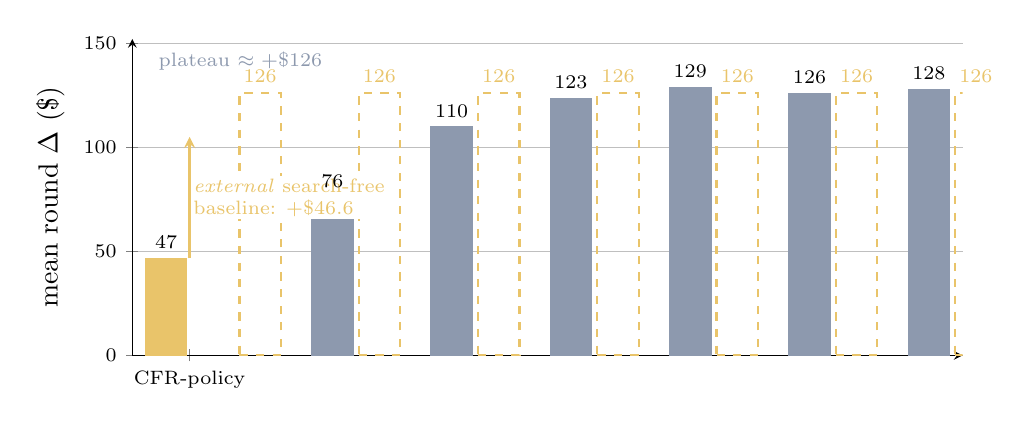
\begin{tikzpicture}
\begin{axis}[
  ybar, bar width=15pt,
  width=\linewidth, height=5.6cm,
  ymin=0, ymax=152,
  ylabel={mean round $\Delta$ (\$)},
  symbolic x coords={CFR-policy,Heuristic,IS-MCTS,M3,M4,P1,P2},
  xtick=data,
  xticklabel style={font=\scriptsize},
  yticklabel style={font=\scriptsize},
  ymajorgrids,
  axis lines=left,
  enlarge x limits=0.08,
  nodes near coords,
  nodes near coords align={anchor=south},
  every node near coord/.append style={font=\scriptsize,
    /pgf/number format/.cd, fixed, precision=0},
]
\addplot[fill=figgiegold, draw=figgiegold, nodes near coords]
  coordinates {(CFR-policy,46.6)};
\addplot[fill=figgiegray, draw=figgiegray]
  coordinates {(Heuristic,76.0) (IS-MCTS,109.8) (M3,123.3) (M4,128.8) (P1,125.8) (P2,127.75)};
\addplot[figgiegold, dashed, thick, forget plot]
  coordinates {(CFR-policy,126)(Heuristic,126)(IS-MCTS,126)(M3,126)(M4,126)(P1,126)(P2,126)};
\node[figgiegray, font=\scriptsize, anchor=south west] at (rel axis cs:0.02,0.87)
  {plateau $\approx +\$126$};
\pgfplotsextra{
  \draw[figgiegold, thick, -stealth] (axis cs:CFR-policy,46.6) --
    node[font=\scriptsize, fill=white, right, inner sep=1pt, align=left]
      {\emph{external} search-free\\baseline: $+\$46.6$} (axis cs:CFR-policy,105);
}
\end{axis}
\end{tikzpicture}
\caption{\textbf{Random-pool benchmark saturates.} Mean round delta vs.\
three random bots (120 rounds, 120 sims, depth 5, seed 7). Labels: CFR-policy
= the search-free reduced-game baseline from \S\ref{sec:cfr} (no neural net,
no search); Heuristic = hand-coded baseline; IS-MCTS = M2 search agent
(heuristic priors); M3--M4, P1, P2 = trained neural checkpoints. The gain
concentrates in the first neural-prior step; later milestones are within
noise.}
\label{fig:random_pool}
\end{figure}

\begin{table}[t]
\centering
\caption{Random-pool benchmark: mean round delta and win share (config:
4 players, 120 ticks, 120 sims, depth 5, seed 7). $\dagger$: training-time
evals at 24 rounds, mean over iterations.}
\label{tab:random_pool}
\begin{tabular}{lrr}
\toprule
Agent & Mean $\Delta$ (\$) & Win share \\
\midrule
Heuristic                       & +76.0   & 0.65 \\
IS-MCTS (M2)                    & +109.8  & 0.85 \\
M3 (neural)                     & +123.3  & 0.95 \\
M4 (population)                 & +128.8  & 0.97 \\
P1 ($+$history)                 & +125.8  & 0.94 \\
P2 ($+$learned belief)          & +127.75 & 0.95 \\
\midrule
CFR-policy (reduced-game, no search) & +46.6 & 0.46 \\
\midrule
P1v (recalibrated)              & +126.8  & 0.98$^{\dagger}$ \\
P1b (bundle)                    & +111.4  & 0.88$^{\dagger}$ \\
\bottomrule
\end{tabular}
\end{table}

\begin{figure}[t]
\centering
\begin{tikzpicture}
\begin{axis}[
  ybar, bar width=7pt,
  width=\linewidth, height=5.8cm,
  ymin=-60, ymax=60,
  ylabel={mean round $\Delta$ (\$)},
  symbolic x coords={M4,P2,P2+combine,P1b},
  xtick=data,
  xticklabel style={font=\scriptsize},
  yticklabel style={font=\scriptsize},
  ymajorgrids,
  axis lines=left,
  enlarge x limits=0.1,
  legend style={at={(0.02,0.98)}, anchor=north west, font=\scriptsize,
    draw=none, legend columns=4},
]
\addplot[fill=figgienavy, draw=figgienavy] table[x=run, y=neural]{data/mixed_pool.dat};
\addplot[fill=figgieteal, draw=figgieteal] table[x=run, y=ismcts]{data/mixed_pool.dat};
\addplot[fill=figgieorange, draw=figgieorange] table[x=run, y=heuristic]{data/mixed_pool.dat};
\addplot[fill=figgiegray, draw=figgiegray] table[x=run, y=random]{data/mixed_pool.dat};
\legend{neural, IS-MCTS, heuristic, random}
\end{axis}
\end{tikzpicture}
\caption{\textbf{Mixed full-pool benchmark.} Mean round delta per seat
(neural + IS-MCTS + heuristic + random; 40 rounds, 100 sims, depth 4, seed
12345). \emph{P2} = learned belief; \emph{P2+combine} = Bayes-combining the
learned belief into the observation; \emph{P1b} = bundle-quote checkpoint.
Behavior conditioning helps only in this pool.}
\label{fig:mixed_pool}
\end{figure}

\subsection{Mixed pool: behavior conditioning pays only here}
\label{sec:r2}

Figure~\ref{fig:mixed_pool} and Table~\ref{tab:mixed_pool} report the mixed
full-pool evaluations. Two consistent measurements show that the learned
belief improves play against behavior-driven opponents: the P2 documentation
measured $+\$24.50$ (no belief) $\to$ $+\$29.75$ (belief), a $+5.25$ gain,
and the controlled A/B at the same config measured the belief-only checkpoint
at $+\$43.25$, rising to $+\$49.00$ when the learned belief is
Bayes-combined into the observation and into world sampling, a further
$+5.75$. The sign of the effect is stable across these runs even though the
absolute level is not; the pattern is that \emph{behavior conditioning only
helps against behavior-driven opponents}. The neural seat wins the pool in
every configuration except the bundle checkpoint (P1b, $\S$\ref{sec:bundle}).

\begin{table}[t]
\centering
\caption{Mixed full-pool benchmark: mean round delta per seat, and neural
win share (40 rounds, 100 sims, depth 4, seed 12345). P2$^\star$ is the
earlier documented run (no controlled seat-wise breakdown).}
\label{tab:mixed_pool}
\begin{tabular}{lrrrrr}
\toprule
Checkpoint & Neural & IS-MCTS & Heuristic & Random & Neural win \\
\midrule
M4                    & +49.3  & +9.5   & $-8.8$   & $-50.0$ & 0.56 \\
P2 (learned belief)   & +43.25 & +7.0   & $-1.5$   & $-48.75$ & 0.53 \\
P2 $+$ Bayes-combine  & +49.00 & +0.58  & $-2.42$  & $-47.17$ & 0.57 \\
P1b (bundle)          & +28.50 & +16.0  & $-1.0$   & $-43.50$ & 0.42 \\
\midrule
P2$^\star$ (no belief) & +24.50 & ---    & ---      & ---      & --- \\
P2$^\star$ (belief)    & +29.75 & ---    & ---      & ---      & --- \\
\bottomrule
\end{tabular}
\end{table}

\subsection{Reduced-game exploitability and a CFR-policy agent}
\label{sec:cfr}

The 4-player game is general-sum, so there is no well-defined Nash
equilibrium and the pool benchmarks above can only establish empirical
domination. To add a game-theoretic measurement, we reduce Figgie to a
two-player, zero-sum subgame, \emph{Figgie-Lite}, and solve it exactly with
chance-sampled counterfactual regret minimization (CFR)
\citep{zinkevich2008regret, lanctot2009mccfr}. Figgie-Lite keeps the
structure that makes the full game hard: a hidden goal suit, a
world-dependent deck (the goal suit appears three times, the others once),
and simultaneous buy-only actions at a fixed price, so a buy is a public
signal. Each tick is resolved in player order (player 0 then player 1) and
the public history records both actions and both buy outcomes. With 4 worlds
$\times$ 8 deals $\times$ 5 actions the tree is small enough to enumerate
both players' actions exactly at every node; the only sampling is the chance
node. The resulting average strategy is a strict improvement over the
hand-crafted references and nearly unexploitable in the reduction.

\begin{table}[t]
\centering
\caption{Figgie-Lite exploitability of the CFR average strategy
($\varepsilon_0+\varepsilon_1$, in payoff units where a goal card is worth
10), and of the reference strategies at two ticks. CFR converges in minutes
on a laptop.}
\label{tab:exploitability}
\begin{tabular}{lrrr}
\toprule
Strategy & Ticks & Iterations & Exploitability \\
\midrule
CFR average & 1 & 60k & 0.0071 \\
CFR average & 2 & 60k & 0.0833 \\
CFR average & 2 & 150k & 0.0425 \\
CFR average & 3 & 40k & 0.0913 \\
\midrule
Reference: pass   & 2 & --- & 12.00 \\
Reference: uniform & 2 & --- & 20.22 \\
Reference: belief-buy & 2 & --- & 5.00 \\
Reference: belief-signals & 2 & --- & 17.00 \\
\bottomrule
\end{tabular}
\end{table}

Exploitability is measured by exact best response. This requires care: the
best-responding player's belief at an info set is a posterior over chance
outcomes that must weight each deal by the opponent's reach along the
\emph{observed} public history (a Bayesian update on the opponent's past
actions). A value-iteration best response that ignored this reach weight
underestimated the reduced-game exploitability by a wide margin; the
corrected backward-pass best response satisfies the bound
$\operatorname{BR}_1 \ge -V_0$ that any best response must, and
$\varepsilon_0,\varepsilon_1 \ge 0$ throughout training
(Table~\ref{tab:exploitability}). The reference strategies are exploitable by
1--4 units per goal card; the CFR average strategy converges to
$\varepsilon \approx 0.04$--0.09, i.e.\ well below one card's value.

To test whether the reduced-game solution transfers to the full engine, we
wrap the two-tick policy in a full-engine agent: an exact posterior over the
goal suit from the private hand selects the target suit, and the CFR policy
for that world gates when to buy (the reduced game's buy-only actions cannot
express the full book, so the agent uses the policy purely as an
aggressiveness signal and works the order book to buy its target). Figure
\ref{fig:cfr_pool} and Table~\ref{tab:cfr_pool} report the result with
round-level bootstrap 95\% confidence intervals, paired Wilcoxon signed-rank
tests, and paired Cohen's $d$ (the deltas are paired because every agent
plays every round under rotated seating). Against three random bots the CFR
agent is clearly positive over three seeds ($+\$40.1$, CI
$[+36.3,+43.7]$, paired diff $+\$50.8$, $p<0.0001$, $d{=}0.43$). In the
mixed full pool (CFR + IS-MCTS + heuristic + random, 120 sims, depth 5),
pooled over three seeds of 80 rounds, it is statistically indistinguishable
from the hand-coded heuristic ($+\$8.1$ vs.\ $+\$11.0$; $p{=}0.61$,
$d{=}{-}0.03$), significantly above random ($p<0.0001$), and significantly
\emph{below} the search agent ($p{=}0.002$, $d{=}{-}0.19$). The single-seed
80-round run on seed 12345 had suggested a second-place finish; pooling over
seeds tightens this to the more precise claim that the reduced policy is
roughly heuristic-level without search. The transfer is partial: the reduced
policy captures the cheap-accumulation behavior but not the ask/sell
subtleties of the full book, matching the finding that buy-only behavior is
the easy part of the game (\S\ref{sec:discussion}).

\begin{figure}[t]
\centering
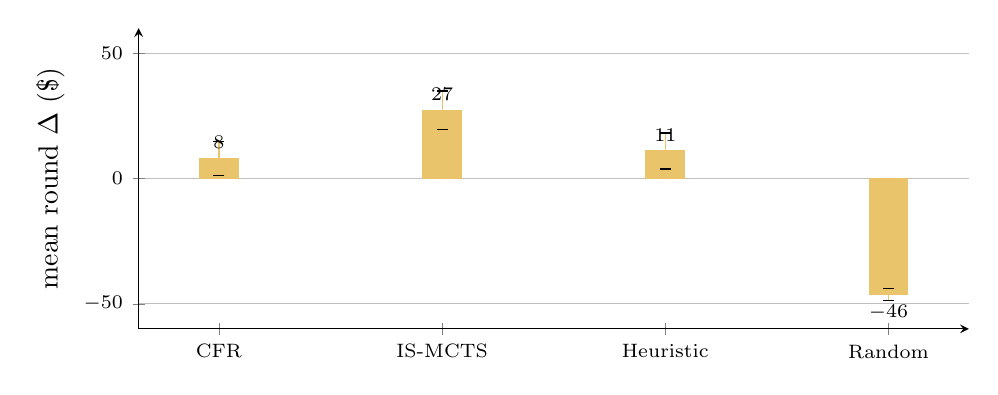
\begin{tikzpicture}
\begin{axis}[
  ybar, bar width=14pt,
  width=\linewidth, height=5.4cm,
  ymin=-60, ymax=60,
  ylabel={mean round $\Delta$ (\$)},
  symbolic x coords={CFR,IS-MCTS,Heuristic,Random},
  xtick=data,
  xticklabel style={font=\scriptsize},
  yticklabel style={font=\scriptsize},
  ymajorgrids,
  axis lines=left,
  enlarge x limits=0.12,
  error bars/y dir=both, error bars/y explicit,
  every node near coord/.append style={font=\scriptsize,
    /pgf/number format/.cd, fixed, precision=0},
]
\addplot[fill=figgiegold, draw=figgiegold, nodes near coords]
  coordinates {(CFR,8.12) +- (0,6.83) (IS-MCTS,27.28) +- (0,7.68)
    (Heuristic,11.00) +- (0,7.20) (Random,-46.40) +- (0,2.44)};
\end{axis}
\end{tikzpicture}
\caption{\textbf{CFR-policy agent in the mixed full pool.} Mean round delta
per seat with bootstrap 95\% CIs (CFR + IS-MCTS + heuristic + random; three
seeds $\times$ 80 rounds, 120 sims, depth 5). The reduced-game policy agent
is statistically indistinguishable from the heuristic and dominates random,
but is below the search agent.}
\label{fig:cfr_pool}
\end{figure}

\begin{table}[t]
\centering
\caption{Mixed full-pool benchmark with the CFR-policy agent: mean round
delta, bootstrap 95\% CI, win share, and paired Wilcoxon signed-rank tests
and Cohen's $d$ of each seat against the CFR seat (three seeds $\times$ 80
rounds, 120 sims, depth 5).}
\label{tab:cfr_pool}
\begin{tabular}{lrrrll}
\toprule
Agent & Mean $\Delta$ (\$) & 95\% CI & Win share & $p$ vs.\ CFR & $d$ \\
\midrule
IS-MCTS & +27.28 & $[+20.0,+35.4]$ & 0.41 & 0.002 & $-0.19$ \\
Heuristic & +11.00 & $[+3.9,+18.3]$ & 0.30 & 0.61 & $-0.03$ \\
CFR     & +8.12 & $[+1.3,+14.9]$  & 0.28 & ---   & --- \\
Random  & $-46.40$ & $[-48.6,-43.7]$ & 0.02 & $<0.0001$ & $+0.94$ \\
\bottomrule
\end{tabular}
\end{table}



\begin{figure}[t]
\centering
\begin{tikzpicture}
\begin{axis}[
  width=\linewidth, height=5.8cm,
  xlabel={mean predicted value $\hat v$},
  ylabel={mean actual value $v$},
  xmin=-1.4, xmax=2.7, ymin=-0.6, ymax=3.1,
  xticklabel style={font=\scriptsize},
  yticklabel style={font=\scriptsize},
  ymajorgrids,
  axis lines=left,
  legend style={at={(0.02,0.98)}, anchor=north west, font=\scriptsize,
    draw=none},
]
\addplot[figgiegray, dashed, thick]
  coordinates {(-0.6,-0.6) (2.6,2.6)}; \addlegendentry{perfect calibration}
\addplot[figgieorange, thick, domain=-1.4:2.7, samples=2]
  {0.22698*x+1.74790}; \addlegendentry{affine fit $y=0.23x+1.75$}
\addplot[only marks, mark=*, mark size=2.6pt, figgienavy]
  table[x=pred, y=actual]{data/calib.dat};
\pgfplotsextra{
  \draw[figgiegray, thin] (axis cs:2.268,2.31) -- (axis cs:1.15,2.62);
  \node[font=\scriptsize, figgiegray, align=center] at (axis cs:1.15,2.62)
    {$n=2276$ (92\%)};
}
\end{axis}
\end{tikzpicture}
\caption{\textbf{Value-head reliability after recalibration (P1v).} Each
point is a prediction bin, sized by the text annotation to its sample count.
After training with full value weight ($w_v{=}1.0$), the top bin moved from
$+1.76 \to +2.28$ (P1, under-scaled) to $+2.27 \to +2.31$; MSE $0.96$, ECE
$0.08$. The curve is dominated by a single large bin ($n{=}2276$, 92\% of
samples) of ``agent wins big'' outcomes, and the raw correlation
(corr$\approx0.2$) remains low; the recalibration is diagnostic rather than
actionable for search.}
\label{fig:calib}
\end{figure}

The scalar value head was diagnosed (M3) to be essentially \emph{constant} in
the liquid random-pool regime: with weight decay it predicts the mean settle
for every observation, corr$\approx0$, because the seat's eventual delta is
dominated by deal and opponent randomness that the 41-float observation
cannot foresee. This is not miscalibration (it is not overconfident on a
learned signal) but \emph{uninformativeness}; PUCT's $q$-term degenerates and
selection is driven by the policy prior. Two interventions change the
picture. First, the \emph{4-player} value head (P1) is genuinely informative
(zeroing it collapses the bench from $+\$111$ to $+\$49.9$), because it
models opponents' payoffs, not just ours. Second, recalibrating the value head
by retraining with full value weight (P1v) restores top-bin calibration:
Figure~\ref{fig:calib} shows the P1v reliability diagram (MSE $0.96$, ECE
$0.08$), the affine artifact ($v \approx 0.23\,\hat v + 1.75$), and the
documented caveat that the fit is dominated by the single ``big win'' bin and
is therefore diagnostic.

\begin{table}[t]
\centering
\caption{Value-head calibration diagnostics. P1v is measured on the dedicated
held-out harness (value\_calibrate.py); other rows are in-training diagnostics
on the growing replay buffer, included for reference.}
\label{tab:calib}
\begin{tabular}{lrrrrr}
\toprule
Checkpoint & MSE & ECE & corr & top-bin $\hat v \to v$ \\
\midrule
P1 (value-w 0.5)  & 2.01 & 0.79 & 0.19 & $+2.01 \to +2.29$ \\
P1v (value-w 1.0) & 0.96 & 0.08 & 0.20 & $+2.27 \to +2.31$ \\
P2 (belief)       & 1.97 & 0.67 & $-0.10$ & $+2.21 \to +1.72$ \\
P1b (bundle)      & 1.29 & 0.18 & 0.10 & $+2.11 \to +2.08$ \\
\bottomrule
\end{tabular}
\end{table}

\subsection{Learned belief}
\label{sec:beliefhead}

The P2 belief head is trained to predict the true assignment $a^*$ from the
observation, and its cross-entropy collapses from $\approx2.5$ to
$\approx0.1$ within the first iterations (Figure~\ref{fig:belief_ce}). The
head \emph{does} learn the hidden state. Two design decisions keep this safe.
First, the belief is \emph{decoupled}: the observation always encodes the
exact strategy-free posterior (the distribution the policy and value heads
were trained on), and the belief head only re-weights \emph{world sampling}
inside the exact-consistent set. Second, Bayes-combining the belief into the
observation (P2b) multiplies the exact posterior by the belief softmax,
$P(a) \propto P_{\mathrm{exact}}(a)\, P_{\mathrm{learned}}(a)$; because both
factors live on the exact-consistent support, impossible worlds stay out,
avoiding the overconfidence trap identified for strong behavioral-likelihood
models in earlier probes. As reported in $\S$\ref{sec:r2}, the learned belief
is a \emph{measurable but pool-specific} win: no effect on the random pool
($+125.7 \to +127.7$ at 30r/40s/d3; $+130.8 \to +126.8$ at 40r/100s/d4,
both within noise), and $+5.25$/$+5.75$ on the mixed pool.

\begin{figure}[t]
\centering
\begin{tikzpicture}
\begin{axis}[
  width=\linewidth, height=5.0cm,
  xlabel={global training step},
  ylabel={belief CE $\mathcal L_b$},
  ymode=log, ymin=0.03, ymax=8,
  xmin=0, xmax=1900,
  xticklabel style={font=\scriptsize},
  yticklabel style={font=\scriptsize},
  ymajorgrids,
  axis lines=left,
]
\addplot[figgieteal, thick, mark=*, mark size=1.5pt]
  table[x=step, y=ce]{data/belief_ce.dat};
\addplot[figgiegray, dashed, thick]
  coordinates {(0,0.1) (1900,0.1)};
\node[font=\scriptsize, figgiegray, anchor=west] at (axis cs:1400,0.28)
  {plateau $\approx 0.1$};
\end{axis}
\end{tikzpicture}
\caption{\textbf{Learned-belief training trajectory (P2).} Belief-head
cross-entropy vs.\ the true assignment, logged every 100 optimizer steps.
Each new self-play batch re-raises the CE; within an iteration it collapses
toward $\approx0.1$, the regime of a calibrated estimator.}
\label{fig:belief_ce}
\end{figure}

\subsection{Bundle quotes: a mechanism-correct negative result}
\label{sec:bundle}

We implemented and fully tested combined two-suit \emph{bundle bids}: a
`BUNDLE$(s_1,s_2,\mathrm{price})$` rests a bid that fills \emph{atomically}
after the per-suit execution loop, paying each seller its own best ask and
consuming both asks together, never trading with the buyer itself and never
partially filling. The observation grows to 53 floats (12 new) and the action
space to 45 (24 new logits, zero-initialized on warm start); four new engine
invariants plus the full suite (48 tests) verify correctness.

The learning outcome is an honest negative result
(Figure~\ref{fig:bundle}). A probe of the trained bundle checkpoint found that
the policy posts bundle bids on 452 of 720 decisions (63\%) yet only 2 of 138
trades fill as bundles (1.4\%). The net learns to \emph{spam cheap
non-crossing bids} (they cost only the turn, and opponents never price
information by moving their asks), so on the mixed pool the bundle checkpoint
regresses to $+\$28.50$ (0.42 win share) against $+\$43.25$ (0.53) for the P2
checkpoint. The mechanism is verified correct; the policy does not learn to
use it profitably. This is evidence for our saturation hypothesis: without
opponents that respond to information, a richer action space just gives the
policy more ways to waste turns.

\begin{figure}[t]
\centering
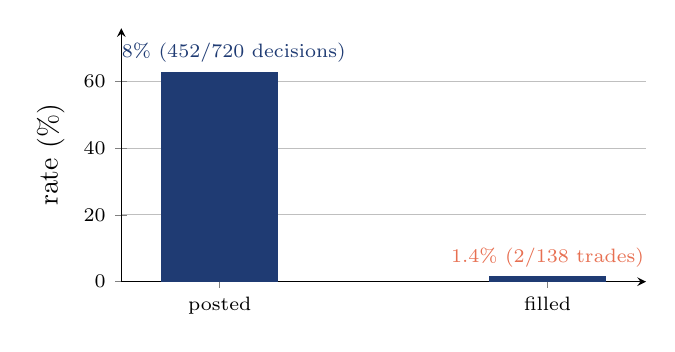
\begin{tikzpicture}
\begin{axis}[
  ybar, bar width=42pt,
  width=0.68\linewidth, height=4.8cm,
  ymin=0, ymax=76,
  ylabel={rate (\%)},
  symbolic x coords={posted,filled},
  xtick=data,
  xticklabel style={font=\scriptsize, align=center},
  yticklabel style={font=\scriptsize},
  ymajorgrids,
  axis lines=left,
  enlarge x limits=0.3,
]
\addplot[fill=figgienavy, draw=figgienavy]
  coordinates {(posted,62.8) (filled,1.4)};
\pgfplotsextra{
  \node[font=\scriptsize, figgienavy, anchor=south] at (axis cs:posted,62.8)
    {62.8\% (452/720 decisions)};
  \node[font=\scriptsize, figgieorange, anchor=south] at (axis cs:filled,1.4)
    {1.4\% (2/138 trades)};
}
\end{axis}
\end{tikzpicture}
\caption{\textbf{Bundle over-posting (P1b).} The policy posts bundle bids on
63\% of turns but fills only 1.4\% of trades as bundles. Combined with the
mixed-pool regression ($+\$28.50$ vs.\ $+\$43.25$), this is an honest negative
result: the mechanism is correct but not learned.}
\label{fig:bundle}
\end{figure}

\subsection{Stability and no-collapse}
\label{sec:r4}

At every training iteration the current checkpoint beat every snapshot it
trained against on the no-collapse check (mean deltas $+\$21$ to $+\$80$
across the pool; win shares $0.33$--$0.83$ on noisy 12-round budgets), and
the random-pool eval held at $+\$120$--$+\$136$ across the population runs.
There is no sign of self-play collapse, and warm-started runs never regress
below the snapshot they started from (see also the validation summary,
\S\ref{sec:vv}).

% ----------------------------------------------------------------------
\section{Discussion and limitations}
\label{sec:discussion}

\paragraph{Why the saturation?} Four facts jointly explain why the
random-pool headline plateaus. (i)~The edge is carried by the \emph{policy
prior} inside search: an untrained net searches worse than the M2
heuristic-prior agent, and the value head is near-constant in the liquid
regime, so the benchmark measures how well the policy learns to buy the
belief-supported suits. A two-layer policy on a 4-price buy grid can reach
that behavior quickly, after which more search or more features add nothing
against opponents that do not react. (ii)~The exact posterior already carries
the flow-consistent signal; the learned belief only adds a refinement that
matters when opponent behavior is informative. (iii)~Action space is
buy-only on a coarse grid; there is no ask/sell/withdraw subtletly to exploit
and no concealment pressure. (iv)~Random opponents never price information,
so the exploration signal for anything beyond cheap accumulation is absent.
This is exactly the setting in which bundle spam (P1b) emerges.

\paragraph{Behavior conditioning is pool-specific.} The most consistent
quantitative result is that belief conditioning (learned belief $+5.25$,
Bayes-combine $+5.75$) helps \emph{only} on the mixed pool. Both effects have
the same sign across runs despite high single-run variance. We interpret this
as the expected general-sum behavior: conditioning matters exactly when
opponents' actions carry information about the hidden state, which heuristic
and search opponents do and random opponents do not.

\paragraph{Generality beyond Figgie.} Our two structural ingredients
\emph{do} transfer to other hidden-information trading games. First, the
exact-belief trick is available in any game whose hidden state is a small,
combinatorially enumerable object: here a $12$-element assignment space, in
general any market with a small set of ``world'' facts (e.g.\ common-value
auctions with a small type profile, or \emph{Hanabi}-style small decks).
Second, the saturation finding is a statement about \emph{opponent
informativeness}, not about Figgie: when the evaluation pool is
behavior-uninformative (random, or any non-adapting opponent), there is no
signal to condition on, and search-with-priors saturates; when opponents
price information, conditioning pays. We expect the same dichotomy in any
negotiation benchmark -- the invariant is that the value of opponent modeling
is bounded by how much opponent \emph{behavior} reveals about the hidden
state. What is Figgie-specific is only the sizes: $T{=}120$ ticks and a
$12$-world assignment space that make exact belief and CPU-scale search
tractable, which is precisely why Figgie is a useful reproducibility
benchmark between toy games and Poker-sized problems.

\paragraph{Limitations.}
\begin{enumerate}[leftmargin=1.5em]
  \item \textbf{Eval scale and variance.} The mixed-pool runs are short
  (40--80 rounds, 100--120 sims, seed 12345) and noisy: the same P2
  configuration measured $+\$24.5$ and $+\$43.25$ across runs. Controlled
  A/B shares a seed, but absolute levels should be read with error bars in
  mind; longer runs (hundreds of rounds) and more seeds are the main
  remaining investment, and are the reason we report bootstrap CIs and
  paired effect sizes rather than point estimates alone. The random-pool
  headline is more stable (120--600 rounds).
  \item \textbf{Internal comparisons only.} All main agents are ours; the
  only external baselines are hand-coded heuristics, the search-free CFR
  policy agent (\S\ref{sec:cfr}), and uniform/random references. We do not
  compare against a general imperfect-information solver such as
  OpenSpiel's CFR/Deep-CFR, which Figgie's simultaneous-move, four-player,
  general-sum structure does not admit directly; the Figgie-Lite reduction
  in \S\ref{sec:cfr} is our attempt to bring the CFR machinery in.
  \item \textbf{Abstraction fidelity.} Buy-only, a 4-price grid, and 120
  discrete ticks abstract away continuous-time negotiation: no queue
  priority, no price-time microstructure, no partial fills. The engine cannot
  express late-round price spikes or concealment through two-sided quoting.
  \item \textbf{Uninformative scalar value.} The value head's low correlation
  limits PUCT's $q$-term; the 4-player head partially restores signal.
  \item \textbf{No exploitability measure in the full game.} For general-sum,
  $n$-player play we can only claim empirical domination of a fixed pool, not
  a game-theoretic guarantee. As a complement, \S\ref{sec:cfr} measures
  exploitability exactly in a two-player zero-sum reduction (Figgie-Lite),
  where the CFR average strategy is nearly unexploitable and a
  reduced-policy agent transfers competitively to the full engine.
  \item \textbf{No human play.} We evaluate against bots only; a human
  baseline (and any qualitative play-testing) is out of scope here.
  \item \textbf{Compute.} CPU training with 24 games/iteration and
  $\sim$40k parameters; larger nets and GPU batches are untested.
\end{enumerate}

\paragraph{Highest-impact next steps.} Ranked by expected impact on
\emph{accuracy}: (1)~an opponent model that reads the agent's own book, which
would force concealment and make bundle spam lose its cheapness;
(2)~an event-driven, continuous-time engine with queue and priority
mechanics; (3)~ask/sell/withdraw actions on a finer price grid, so the agent
can express and exploit two-sided beliefs; (4)~more search with calibrated
values, which becomes worthwhile once features and belief carry signal.

\section{Conclusion}
\label{sec:conclusion}

We presented a complete DRL methodology for Figgie: exact belief tracking,
information-set search, neural priors, population self-play, and a measured
results section with one central and two auxiliary findings, all backed by a
property-verified engine and validated components (\S\ref{sec:vv}). The central
finding is saturation: on the random-pool benchmark the agent reaches
$\sim$95--97\% win share and $\sim$$+\$126\pm5$ mean round delta by M3/M4,
and later modules do not move it, while the same modules deliver consistent
gains ($+5.25$, $+5.75$) against a mixed behavior-driven pool. The auxiliary
findings are honest negatives: bundle quoting is mechanism-correct but not
learned, and the scalar value head is uninformative in the liquid regime but
recalibratable. A two-player zero-sum reduction (Figgie-Lite) adds a
game-theoretic measurement: CFR converges there to near-zero exploitability,
and a policy agent trained on the reduction transfers competitively to the
full pool (\S\ref{sec:cfr}). The released harness (engine with 48 passing
invariant tests, belief tracker, agents, trainer, and seed-configurable evals)
makes every number in this paper reproducible.

Taken together, the results suggest a sharper hypothesis than ``our method
improves play'': \emph{in negotiation games, the bottleneck is not stronger
search but richer opponent models.} Once cheap accumulation is learned, the
remaining headroom is determined by how much information opponents' behavior
reveals about the hidden state -- exactly the axis on which belief
conditioning helped and bundle spam failed. We conjecture that future
progress in hidden-information trading games will come less from deeper
search or larger networks and more from models that read opponent behavior --
and the released harness is designed so that the next iteration of such a
model can be tested immediately.

% ----------------------------------------------------------------------
\section*{Reproducibility}
\noindent
All experiments use frozen checkpoints and seed-configurable evaluators in the
released repository. The manuscript records the evaluation configurations and
fixed seeds used for each comparison. Figure source values are mirrored in
\texttt{paper/make\_figures.py}; hyperparameters are in
Appendix~\ref{app:hparams}. The reported results remain simulator-based and
should be rerun before making claims beyond this environment.

\appendix
\section{Hyperparameters}
\label{app:hparams}

\begin{table}[h]
\centering
\caption{Hyperparameters (as used in the reported runs).}
\label{tab:hparams}
\begin{tabular}{ll}
\toprule
Parameter & Value \\
\midrule
Ticks per round & 120 \\
Players & 4 \\
Price grid & $\{6,12,18,24\}$ (buy-only) \\
Actions (base / +bundle) & 21 / 45 \\
Observation (base / +bundle) & 41 / 53 floats \\
Trunk & 2$\times$128 ReLU, $\sim$40k params \\
History pathway & MLP (P1) / single-head attention $5\to32$ (P2) \\
Search simulations $W$ & 30--120 (eval 120; train 50) \\
Search depth $D$ & 3--5 (eval 5; train 4) \\
PUCT $c_{\mathrm{puct}}$ & 1.0 \\
Self-play games / iteration & 24 \\
Optimizer steps / iteration & $\sim$400 \\
Optimizer & Adam, lr $10^{-3}$, wd $10^{-4}$ \\
Batch & 512 \\
Value weight $w_v$ & 0.5 (P1/P2/P1b), 1.0 (P1v) \\
Belief weight $w_b$ & 0.5 (P2 line), 0 otherwise \\
Opponent mixture & self 0.25, past 0.35, heuristic 0.25, random 0.15 \\
Pool size & 4 snapshots \\
Random-pool eval & 120 rounds, 120 sims, depth 5, seed 7 \\
Mixed-pool eval & 40 rounds, 100 sims, depth 4, seed 12345 \\
CFR eval & random pool 600 rounds / mixed pool 80 rounds, 120 sims, depth 5 \\
Figgie-Lite CFR & 2--3 ticks, 40--150k iterations, buy-only \\
\bottomrule
\end{tabular}
\end{table}

\section{Artifacts}
\label{app:artifacts}
\begin{itemize}[leftmargin=1.5em]
  \item \texttt{src/env}: discretized simultaneous-move engine, deck, order
  book, observations; 48 passing property tests including the four bundle
  invariants and payout conservation.
  \item \texttt{src/belief}: exact assignment posterior (DP over deals) and
  consistent-world sampler.
  \item \texttt{src/agents}: random, heuristic, IS-MCTS, neural (with
  \texttt{learned\_\hspace{0pt}belief} and \texttt{bayes\_\hspace{0pt}combine}
  flags), human playable CLI.
  \item \texttt{src/learning}: FiggieNet, replay, self-play, population
  trainer (including \texttt{load\_\hspace{0pt}partial} architecture growth).
  \item \texttt{experiments/checkpoints}: frozen snapshots \texttt{m4},
  \texttt{p1}, \texttt{p1v}, \texttt{p2}, \texttt{p1b} plus the P1v
  calibration artifact.
  \item \texttt{paper/}: this document, figure data, and
  \texttt{make\_figures.py}.
\end{itemize}

% ----------------------------------------------------------------------
\bibliographystyle{plainnat}
\bibliography{references}

\end{document}
